\section{Methodology}
\label{sec:methodology}

\subsection{Overall System Architecture}

FedRouteAI is an end-to-end, privacy-preserving federated learning framework for multi-class traffic anomaly detection. The system decouples inference from aggregation: all raw telemetry processing and local model training remain at the edge, and only 12.96\,KB model weight payloads are ever transmitted to the central server. Fig.~\ref{fig:architecture} illustrates the complete pipeline across six functional layers.

\begin{figure*}[t]
  \centering
  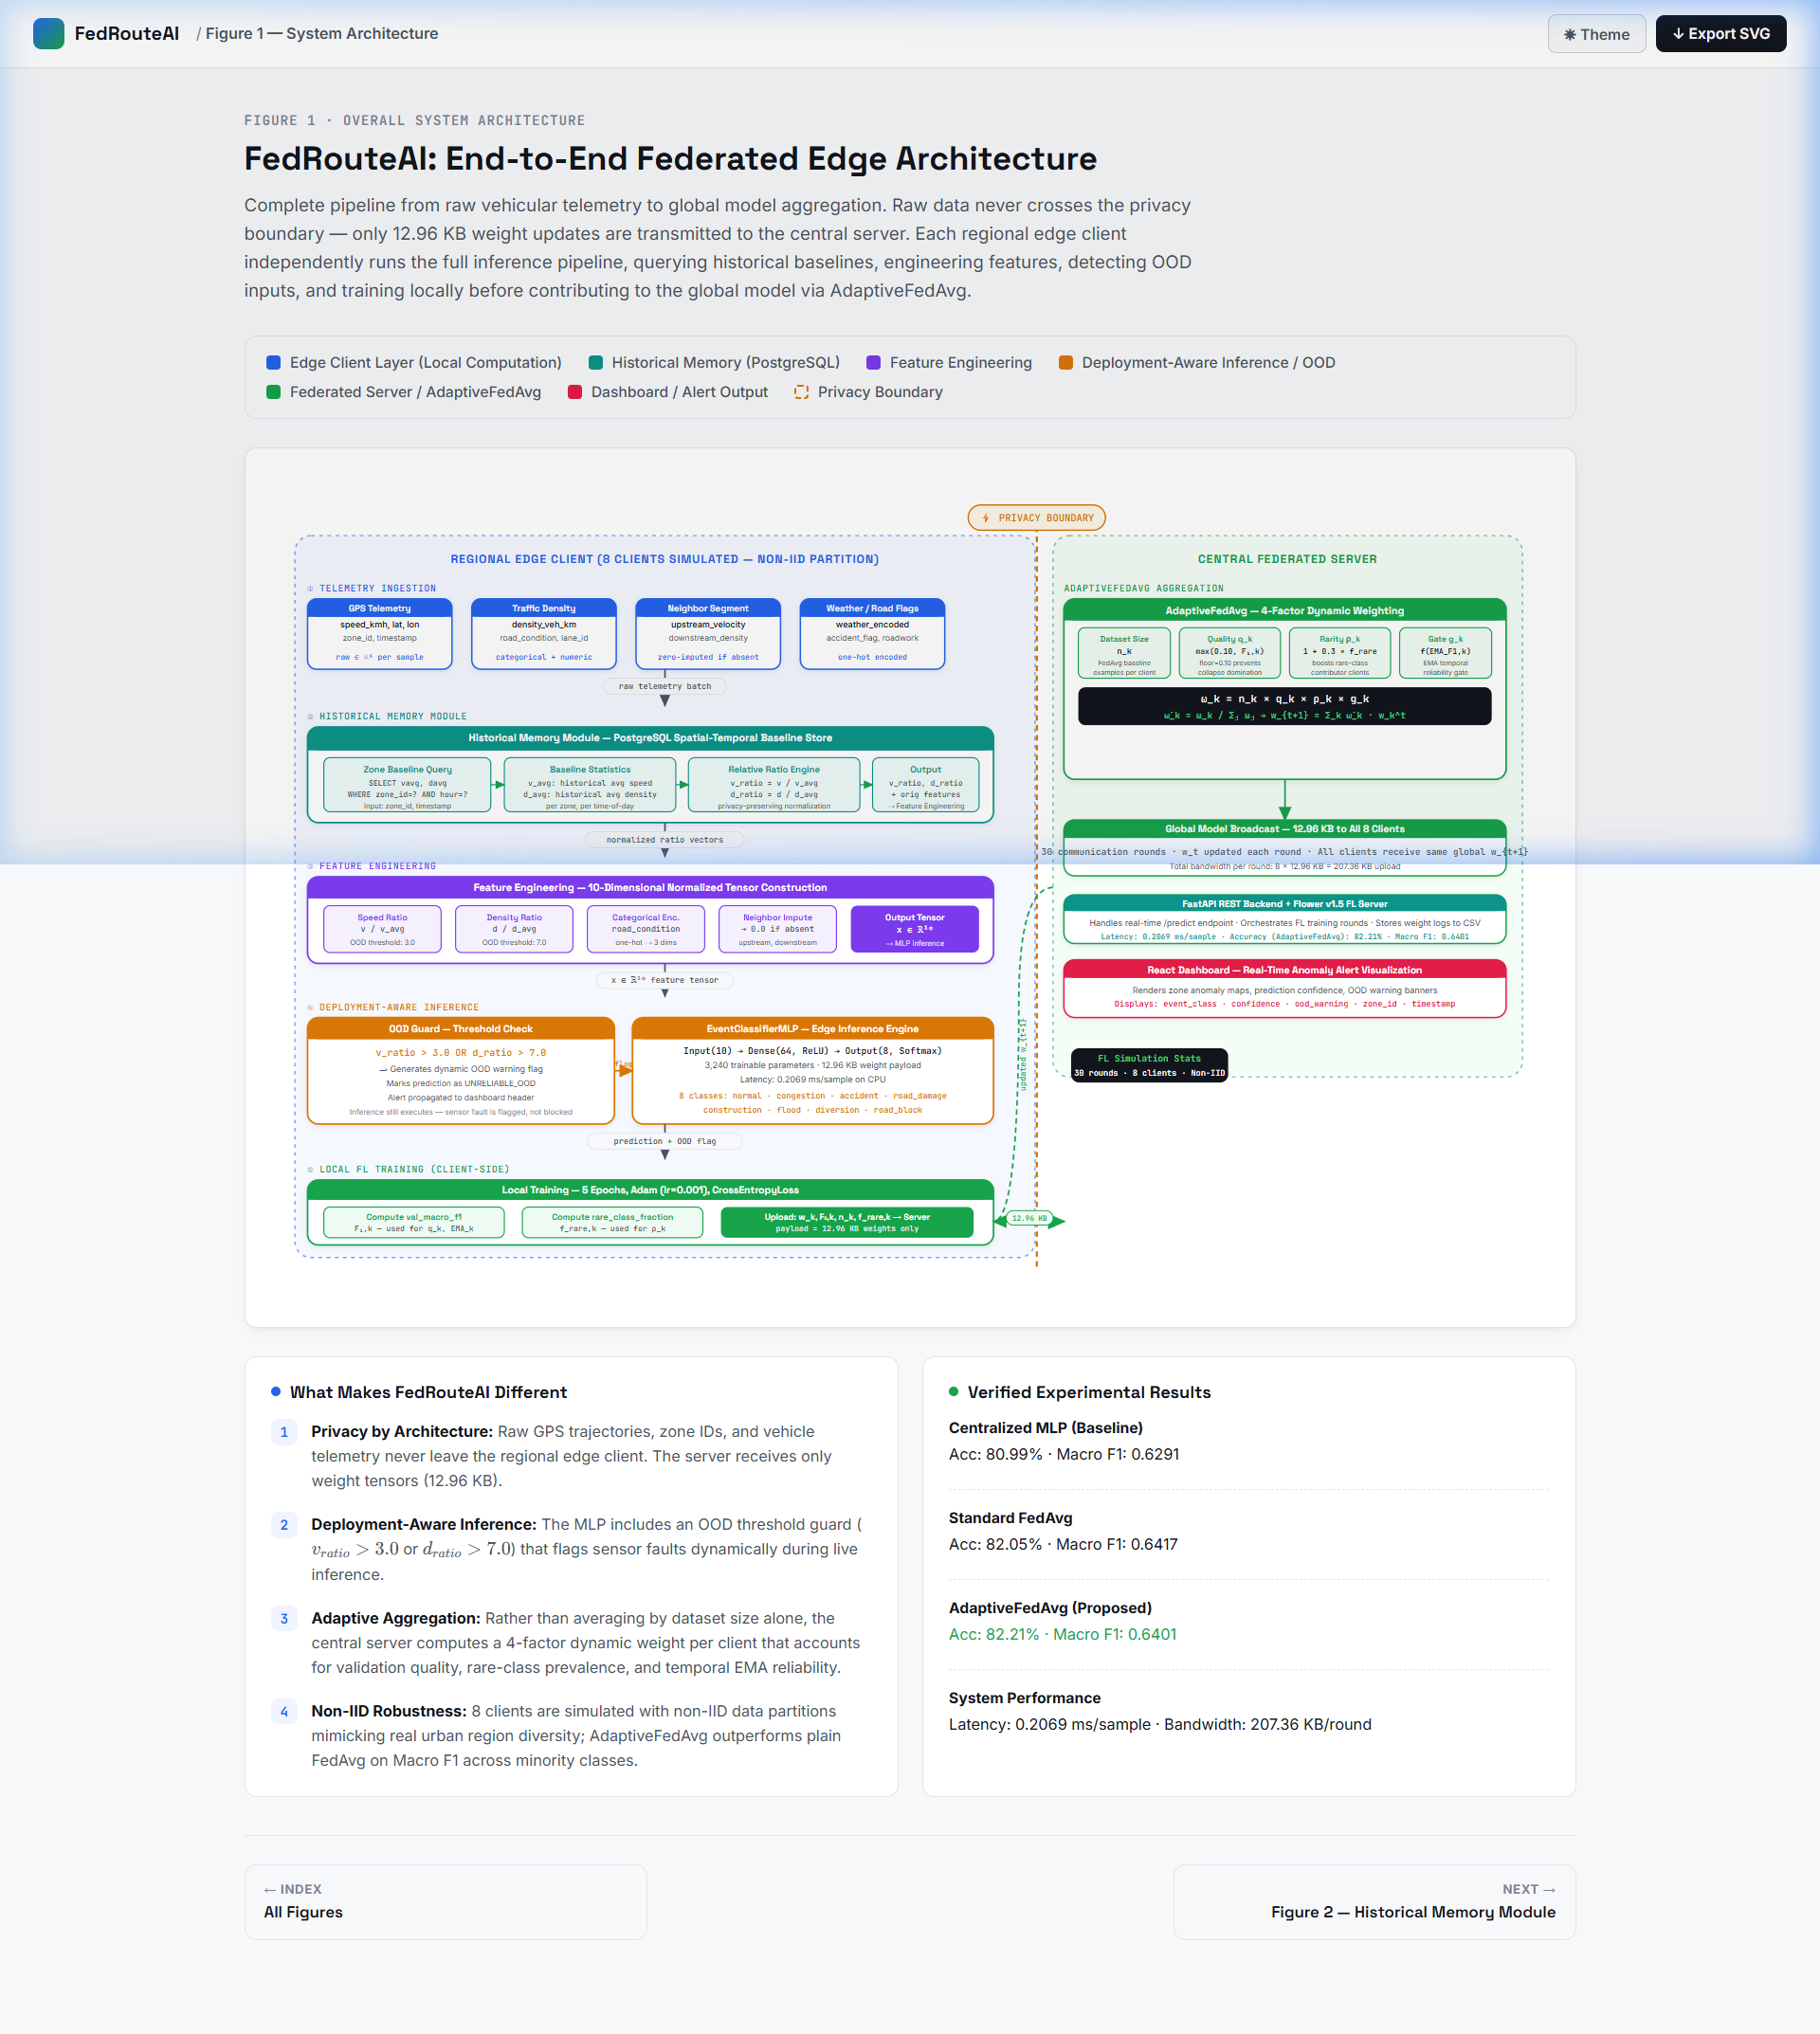
\includegraphics[width=0.95\textwidth]{figures/fig1_system_architecture.png}
  \caption{End-to-end FedRouteAI architecture. Raw GPS telemetry is processed entirely within the regional edge client (blue zone). Only 12.96\,KB model weights cross the privacy boundary (orange dashed line) to the central federated server (green zone). The six functional layers are: telemetry ingestion, Historical Memory normalization, feature engineering, deployment-aware MLP inference, AdaptiveFedAvg aggregation, and the React alerting dashboard.}
  \label{fig:architecture}
\end{figure*}

From an engineering perspective, the framework is orchestrated by a FastAPI backend interfacing with a PostgreSQL database for real-time telemetry ingestion. A React-based visualization dashboard displays live anomaly alerts across simulated geographical zones. The Flower~\cite{Beutel_2020} federated learning server manages communication rounds and model distribution.

The primary research contributions reside within two components: (1) a deployment-aware inference pipeline at the edge that handles real-world sensor degradation, and (2) an adaptive federated aggregation algorithm at the server that accounts for heterogeneous client quality.

\subsection{Historical Memory Module and Feature Engineering}

Directly classifying raw GPS telemetry poses privacy risks and generalization challenges, since absolute speed values differ across urban zone typologies (e.g., residential streets versus motorways). To resolve this, the \emph{Historical Memory Module}---implemented as a PostgreSQL spatial-temporal baseline store---maintains aggregated speed and density statistics per zone and per time-of-day slot~\cite{Chen_2016}.

Fig.~\ref{fig:historical_memory} details the module's internal dataflow. When an edge device records an instantaneous telemetry tuple $(v, d, \text{zone\_id}, t)$, the system queries the baseline store to retrieve historical averages $v_{avg}(\text{zone}, \text{hour})$ and $d_{avg}(\text{zone}, \text{hour})$. Two normalized relative ratios are then computed:

\begin{equation}
  v_{ratio} = \frac{v}{v_{avg}}, \qquad d_{ratio} = \frac{d}{d_{avg}}
  \label{eq:ratios}
\end{equation}

A ratio of 1.0 indicates current conditions are at historical norm; values significantly above 1.0 flag anomalous deviations. Critically, the ratio representation replaces absolute GPS coordinates with deviation-from-norm values, preserving V2X privacy: a speed ratio of 1.24 reveals nothing about a vehicle's absolute position.

\begin{figure}[htbp]
  \centering
  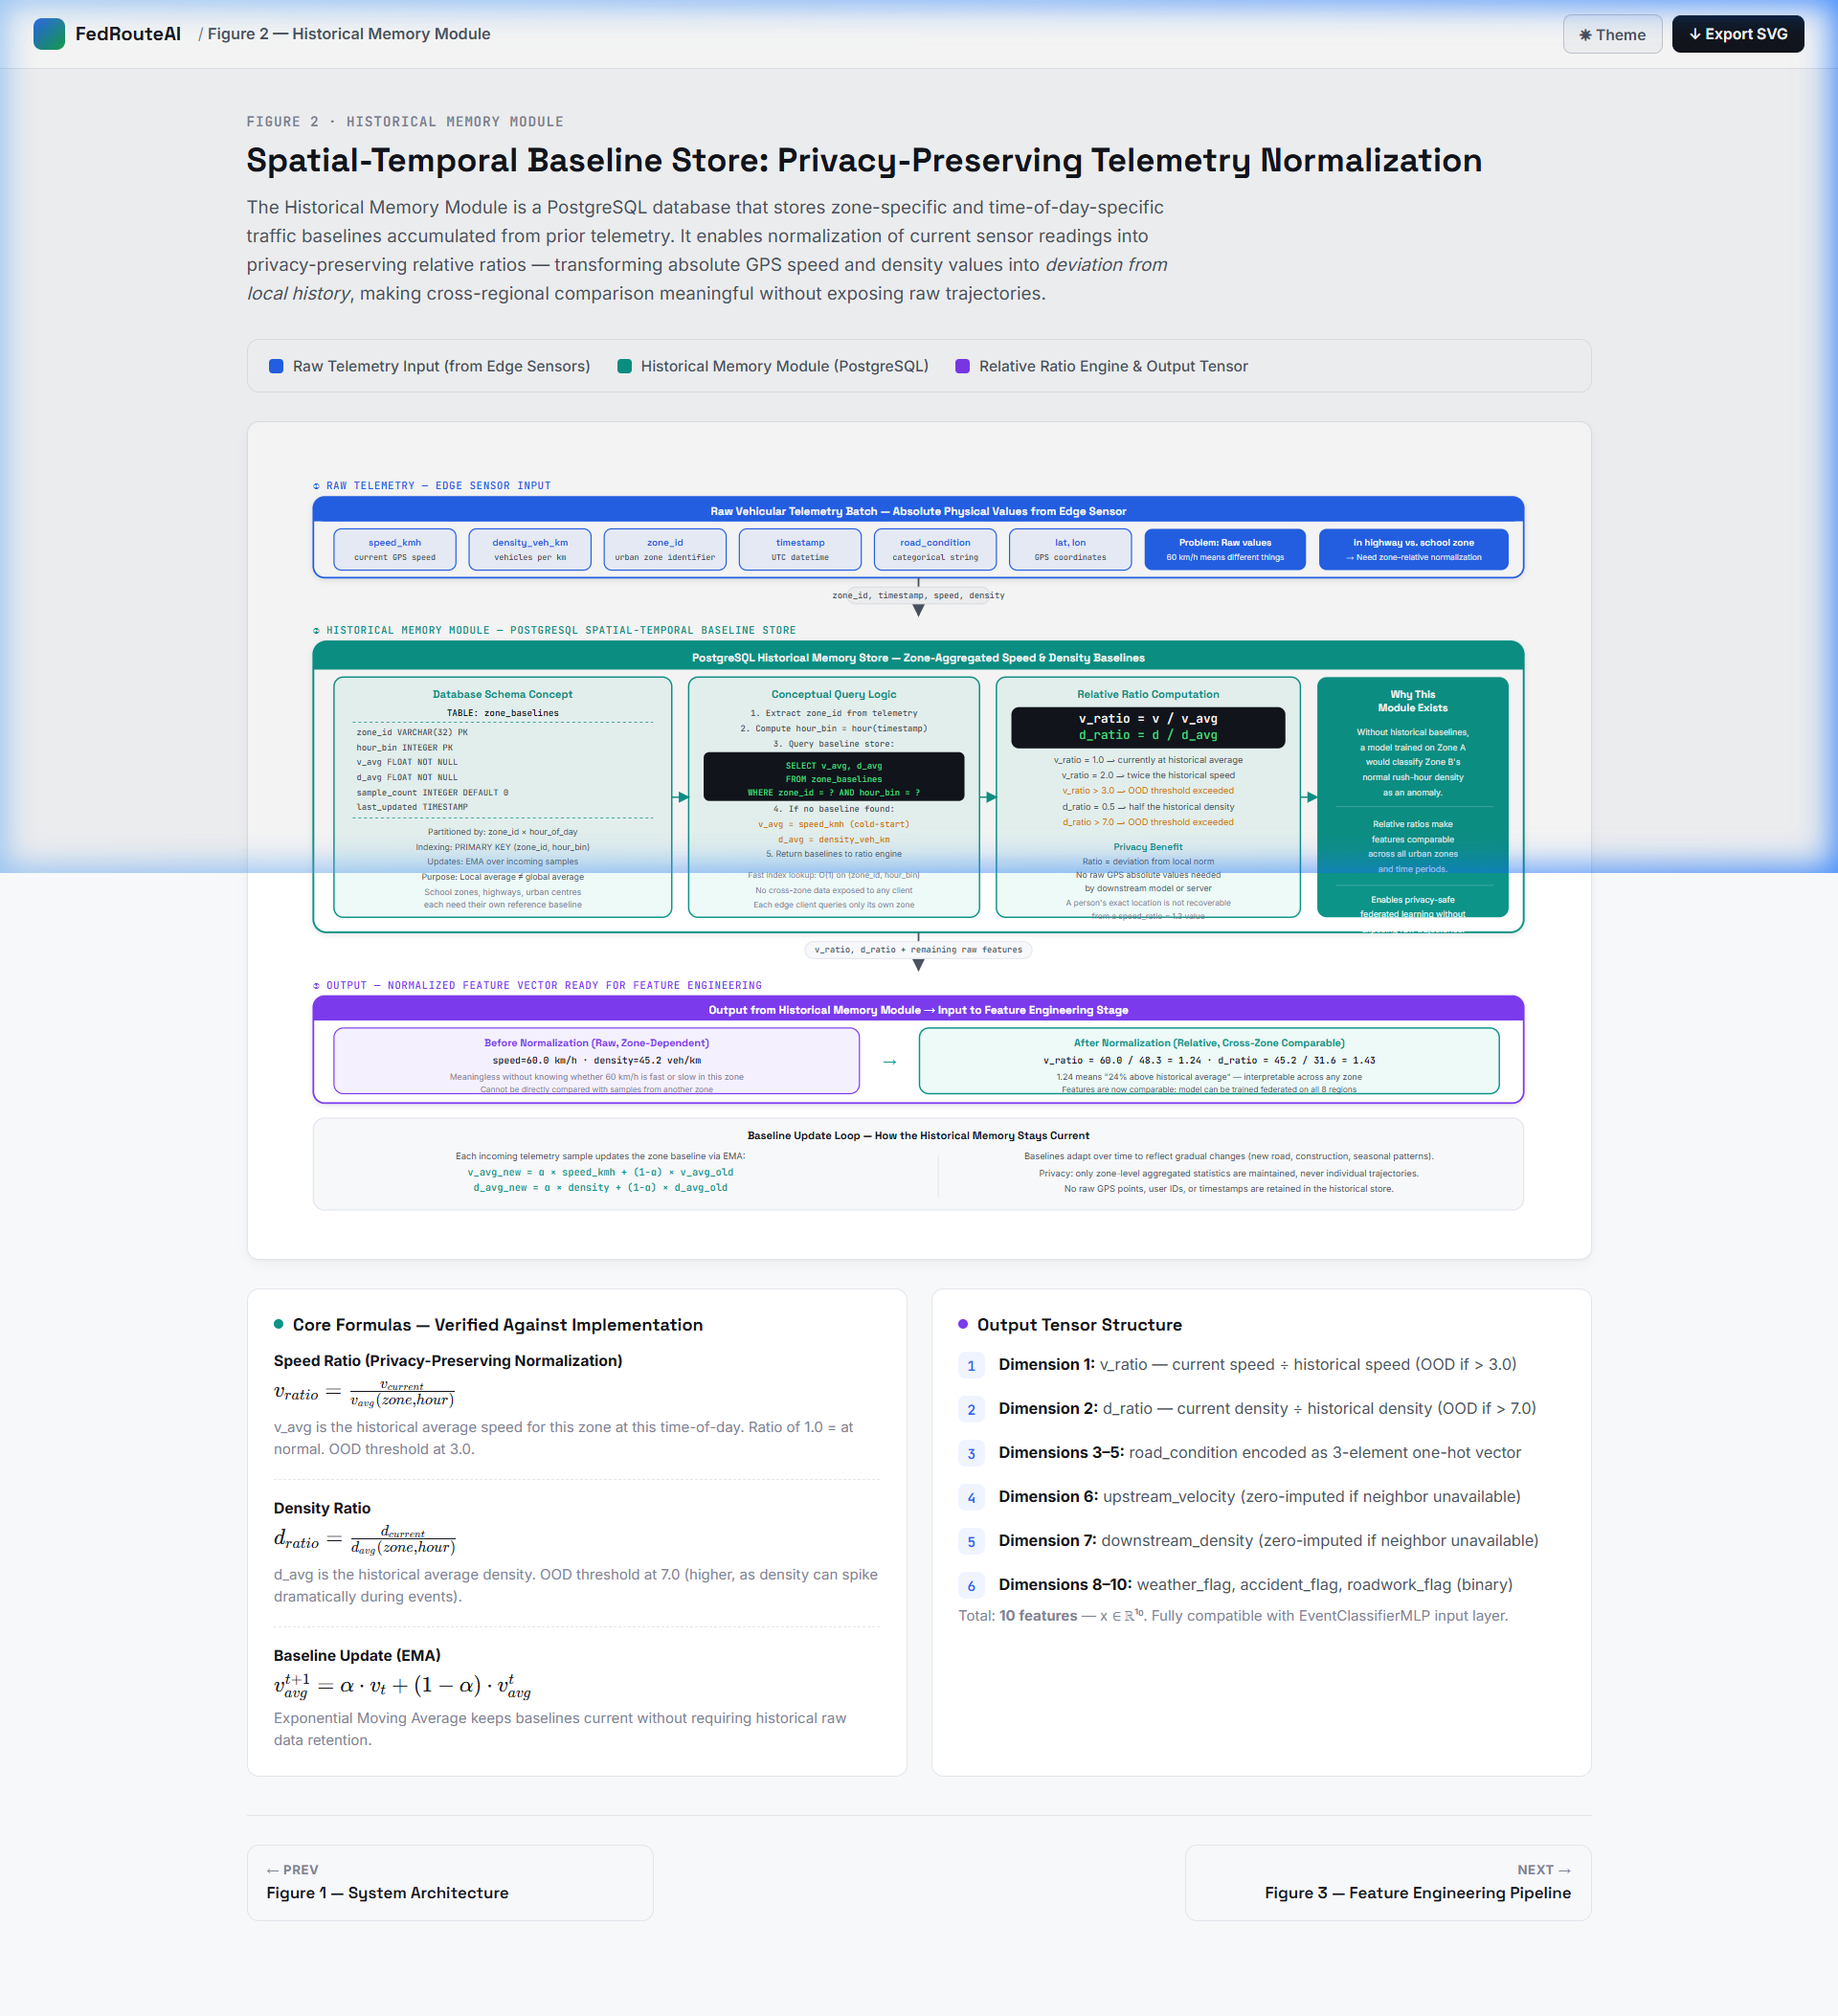
\includegraphics[width=\linewidth]{figures/fig2_historical_memory.png}
  \caption{Historical Memory Module dataflow. Raw telemetry is normalized against zone-specific PostgreSQL baselines to produce privacy-preserving relative ratios $v_{ratio}$ and $d_{ratio}$. The module employs EMA-based baseline updates to track gradual temporal shifts in zone traffic patterns.}
  \label{fig:historical_memory}
\end{figure}

The subsequent feature engineering stage transforms these ratios alongside categorical and neighbor data into a standardized 10-dimensional tensor $\mathbf{x} \in \mathbb{R}^{10}$, as illustrated in Fig.~\ref{fig:feature_engineering}. The five parallel transformation streams are:

\begin{enumerate}
  \item \textbf{Speed ratio} $x[0]$: $v / v_{avg}$ (OOD threshold: $>3.0$)
  \item \textbf{Density ratio} $x[1]$: $d / d_{avg}$ (OOD threshold: $>7.0$)
  \item \textbf{Road condition} $x[2\text{--}4]$: three-element one-hot encoding (dry, wet, snow)
  \item \textbf{Neighbor segment} $x[5\text{--}6]$: upstream velocity, downstream density (zero-imputed if unavailable)
  \item \textbf{Environmental flags} $x[7\text{--}9]$: weather encoding, accident flag, roadwork flag (binary)
\end{enumerate}

\begin{figure}[htbp]
  \centering
  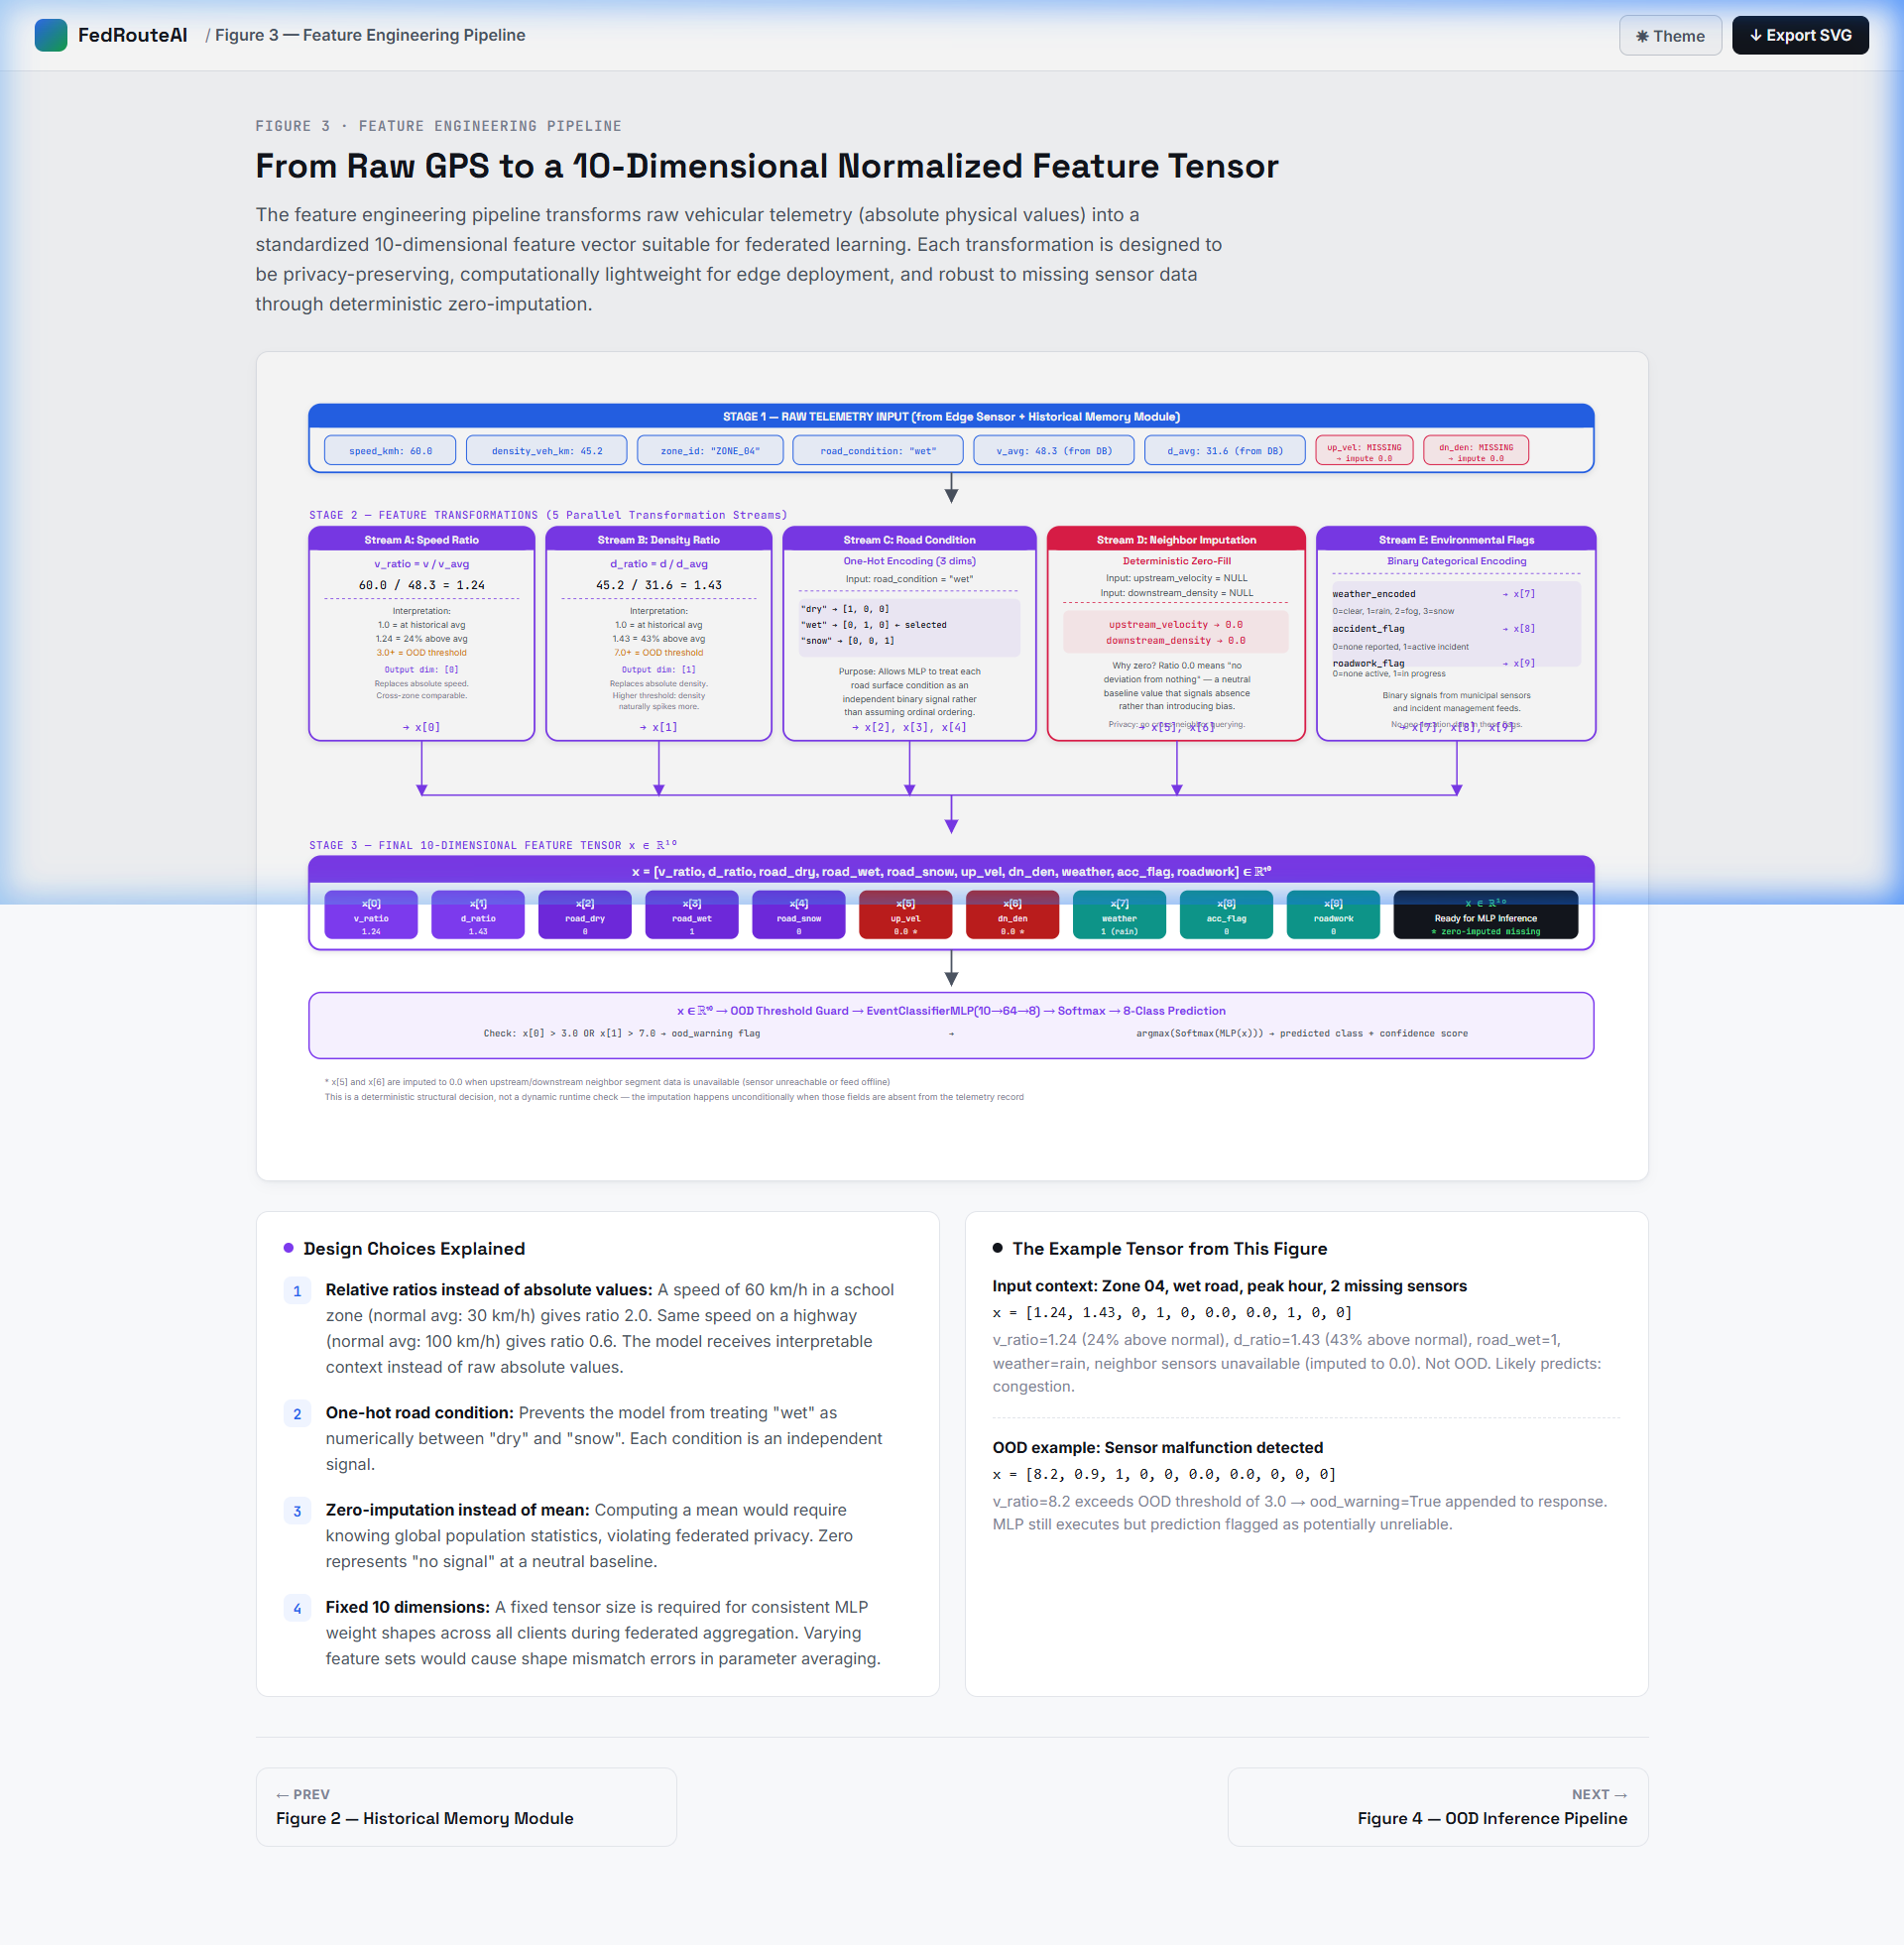
\includegraphics[width=\linewidth]{figures/fig3_feature_engineering.png}
  \caption{Feature engineering pipeline producing $\mathbf{x} \in \mathbb{R}^{10}$ from five parallel transformation streams. Neighbor segment dimensions (dims 5--6) are zero-imputed when sensor feeds are unavailable, mapping missing data to a neutral baseline without requiring global population statistics.}
  \label{fig:feature_engineering}
\end{figure}

The fixed 10-dimensional tensor is required for consistent parameter shapes during federated aggregation: a varying feature count would cause dimension mismatches when averaging client weights.

\subsection{Deployment-Aware Inference and OOD Mitigation}

The central methodological contribution of FedRouteAI is its \emph{deployment-aware inference pipeline}, designed to handle the volatile data environments of live ITS deployments. Traditional neural architectures produce confident but unreliable predictions when fed out-of-distribution (OOD) inputs arising from faulty sensors or extreme environmental conditions~\cite{Hendrycks_2017}.

Fig.~\ref{fig:ood_pipeline} illustrates the two-zone architecture. The main inference path always executes. Simultaneously, a lightweight threshold guard checks the two ratio features:

\begin{equation}
  \text{ood\_flag} = \mathbb{1}[v_{ratio} > 3.0] \;\vee\; \mathbb{1}[d_{ratio} > 7.0]
  \label{eq:ood}
\end{equation}

If either condition is triggered, the pipeline generates a dynamic OOD warning flag that is propagated to the downstream dashboard without blocking inference. Missing neighbor segment data is handled via \emph{deterministic zero-imputation}: mapping absent values to 0.0 represents ``no deviation from a neutral baseline'' and requires no cross-client data sharing, unlike mean imputation.

\begin{figure}[htbp]
  \centering
  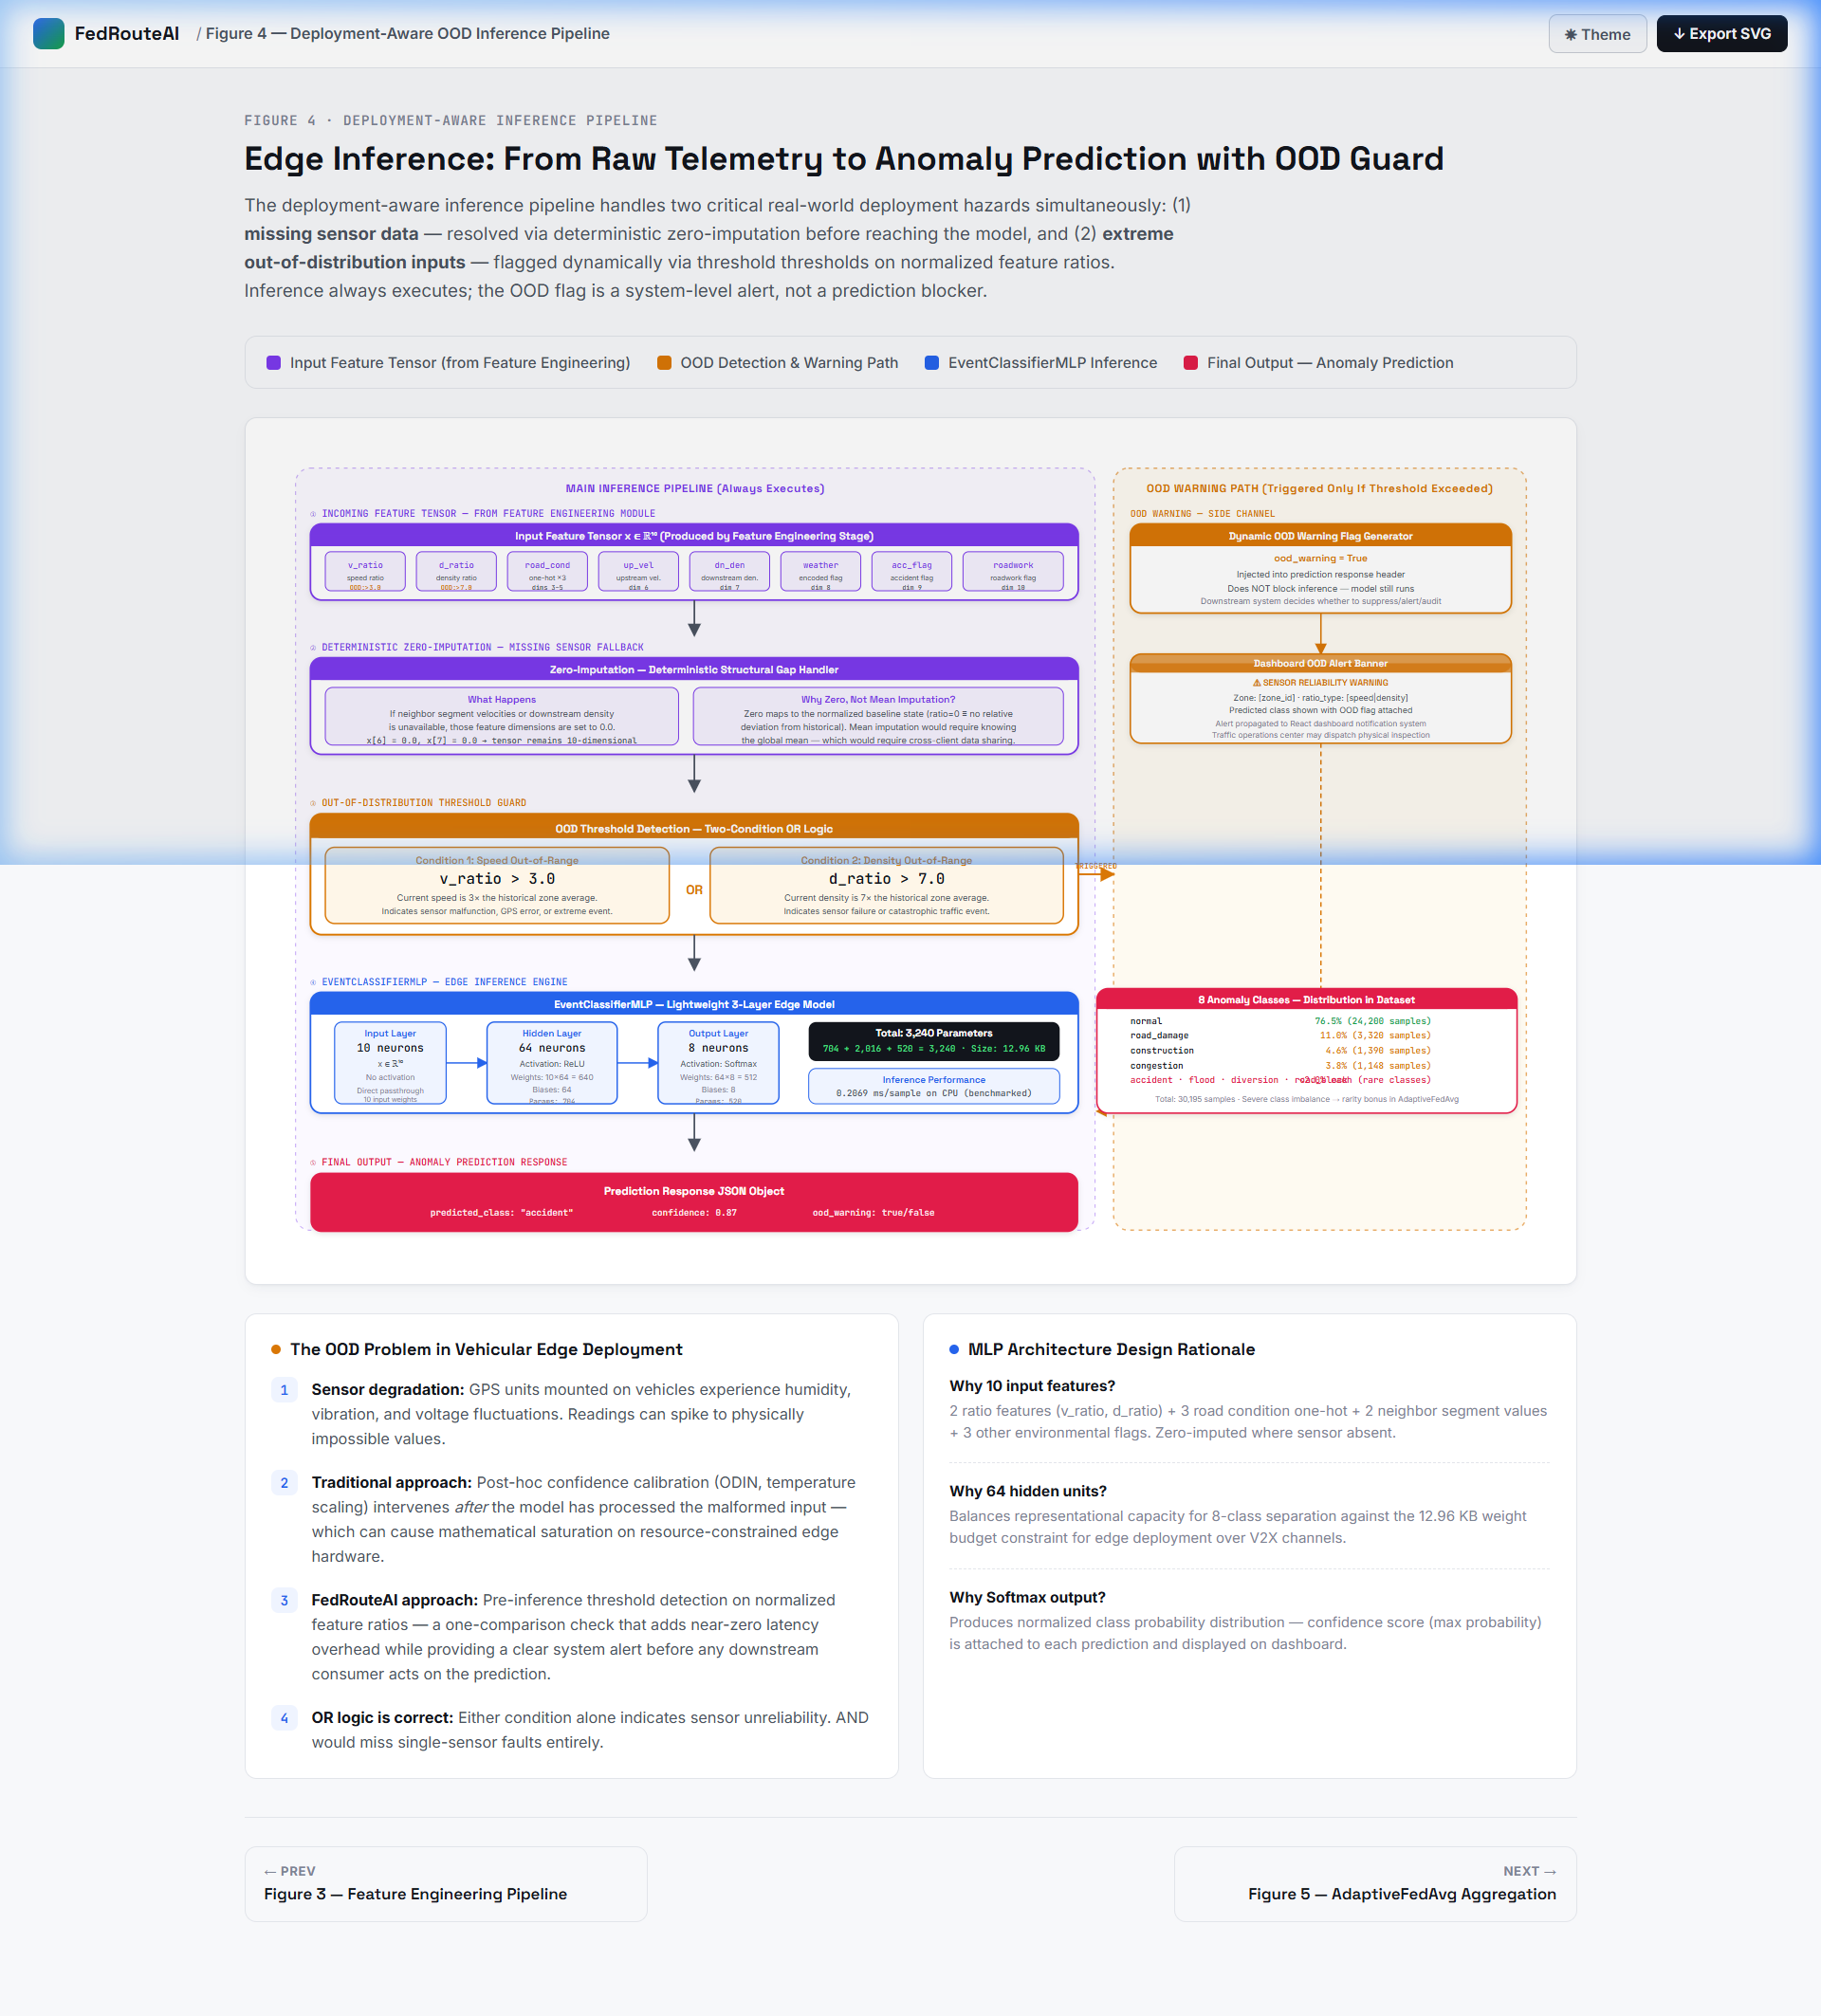
\includegraphics[width=\linewidth]{figures/fig4_ood_pipeline.png}
  \caption{Deployment-aware inference pipeline. The main path processes $\mathbf{x} \in \mathbb{R}^{10}$ through zero-imputation and the EventClassifierMLP at all times (0.2069\,ms/sample). A concurrent OOD side-channel checks Eq.~(\ref{eq:ood}) and injects a warning flag into the response without suppressing the prediction.}
  \label{fig:ood_pipeline}
\end{figure}

The \emph{EventClassifierMLP} edge model has a minimal architecture chosen for V2X deployment:
\[
\text{Input}(10) \;\to\; \text{Dense}(64,\,\text{ReLU}) \;\to\; \text{Output}(8,\,\text{Softmax})
\]
with 3,240 trainable parameters (12.96\,KB as float32). The eight output classes correspond to: \texttt{normal}, \texttt{congestion}, \texttt{accident}, \texttt{road\_damage}, \texttt{construction}, \texttt{flood}, \texttt{diversion}, and \texttt{road\_block}.

\subsection{Adaptive Federated Aggregation}

Standard FedAvg~\cite{McMahan_2017} weights client contributions solely by dataset size, implicitly assuming equal data quality across clients. In vehicular edge environments, this assumption fails: clients with faulty sensors or poor local training quality can degrade the global model.

The proposed \emph{AdaptiveFedAvg} algorithm computes a four-factor dynamic weight $\omega_k$ for each client $k$:

\begin{equation}
  \omega_k = n_k \cdot q_k \cdot \rho_k \cdot g_k
  \label{eq:adaptivefedavg_weight}
\end{equation}

where the four factors are:

\begin{itemize}
  \item $n_k$: dataset size (baseline FedAvg factor)
  \item $q_k = \max(q_{floor},\, F_{1,k})$: floored quality factor, with $q_{floor}=0.10$ preventing model-collapse clients from being completely ignored
  \item $\rho_k = 1.0 + \beta \cdot f_{rare}^k$: rarity bonus with $\beta=0.30$, amplifying clients that hold locally rare anomaly classes (e.g., flood, accident)
  \item $g_k = f(\text{EMA}_{F_1}^k)$: EMA-based temporal reliability gate, bounded in $[g_{min},\, 1.0]$ with $g_{min}=0.50$ and stability threshold $\tau=0.15$
\end{itemize}

The gate function $f(\cdot)$ is defined as:
\begin{equation}
  g_k = \begin{cases} 1.0 & \text{if } \text{EMA}_{F_1}^k \geq \tau \\ g_{min} + (1-g_{min}) \cdot \dfrac{\text{EMA}_{F_1}^k}{\tau} & \text{otherwise} \end{cases}
  \label{eq:gate}
\end{equation}

The EMA is updated each round: $\text{EMA}_{F_1}^k \leftarrow \alpha \cdot F_{1,k} + (1-\alpha) \cdot \text{EMA}_{F_1}^k$ with $\alpha=0.30$. Weights are normalized to a valid convex combination: $\hat{\omega}_k = \omega_k / \sum_j \omega_j$, enforcing $\sum_k \hat{\omega}_k = 1.0$ (verified by assertion in code). The global model update is then:

\begin{equation}
  w_{t+1} = \sum_{k \in \mathcal{K}} \hat{\omega}_k \cdot w_k^{(t+1)}
  \label{eq:global_update}
\end{equation}

Fig.~\ref{fig:adaptivefedavg_workflow} shows the complete server-side aggregation flow, and Fig.~\ref{fig:fl_communication} details the per-round communication protocol. Algorithm~\ref{alg:adaptivefedavg} provides the full pseudocode.

\begin{figure}[htbp]
  \centering
  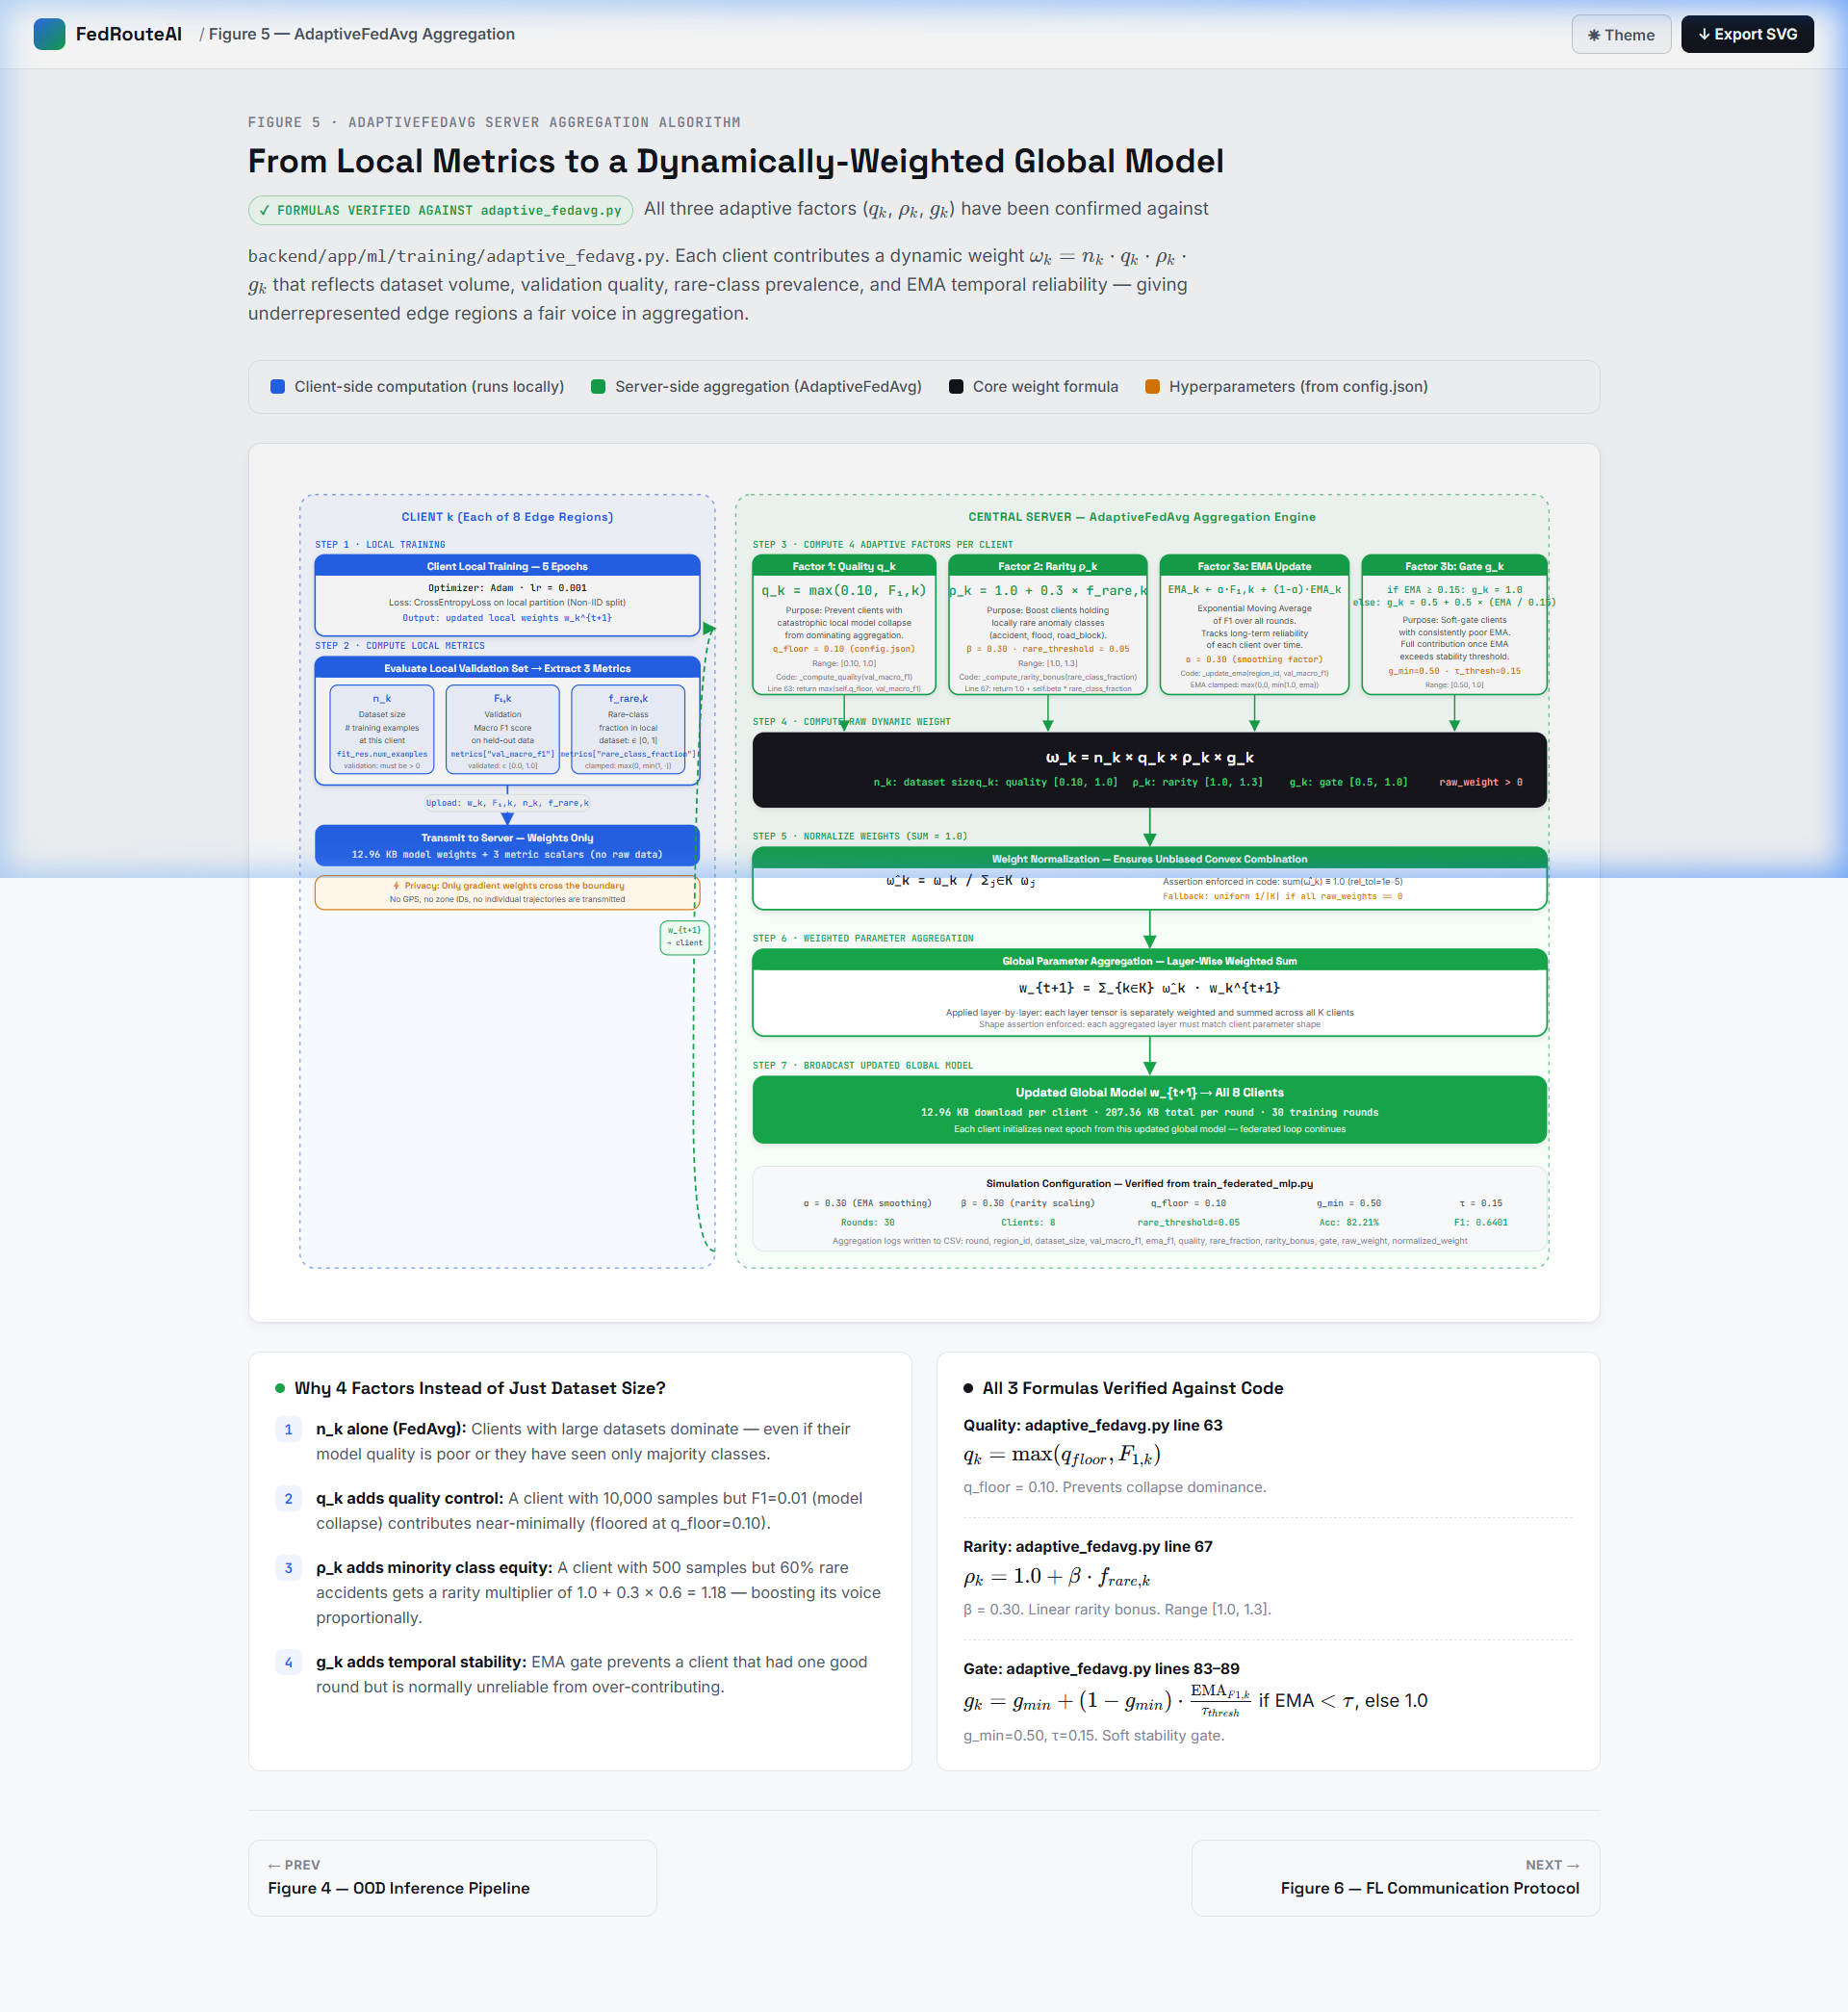
\includegraphics[width=\linewidth]{figures/fig5_adaptivefedavg.png}
  \caption{AdaptiveFedAvg server-side aggregation workflow (7 steps). Client metrics ($n_k$, $F_{1,k}$, $f_{rare}^k$) drive four parallel factor computations, which are combined into a normalized weight vector and applied layer-wise to produce the updated global model $w_{t+1}$. All three formulas are verified against \texttt{adaptive\_fedavg.py}.}
  \label{fig:adaptivefedavg_workflow}
\end{figure}

\begin{figure*}[t]
  \centering
  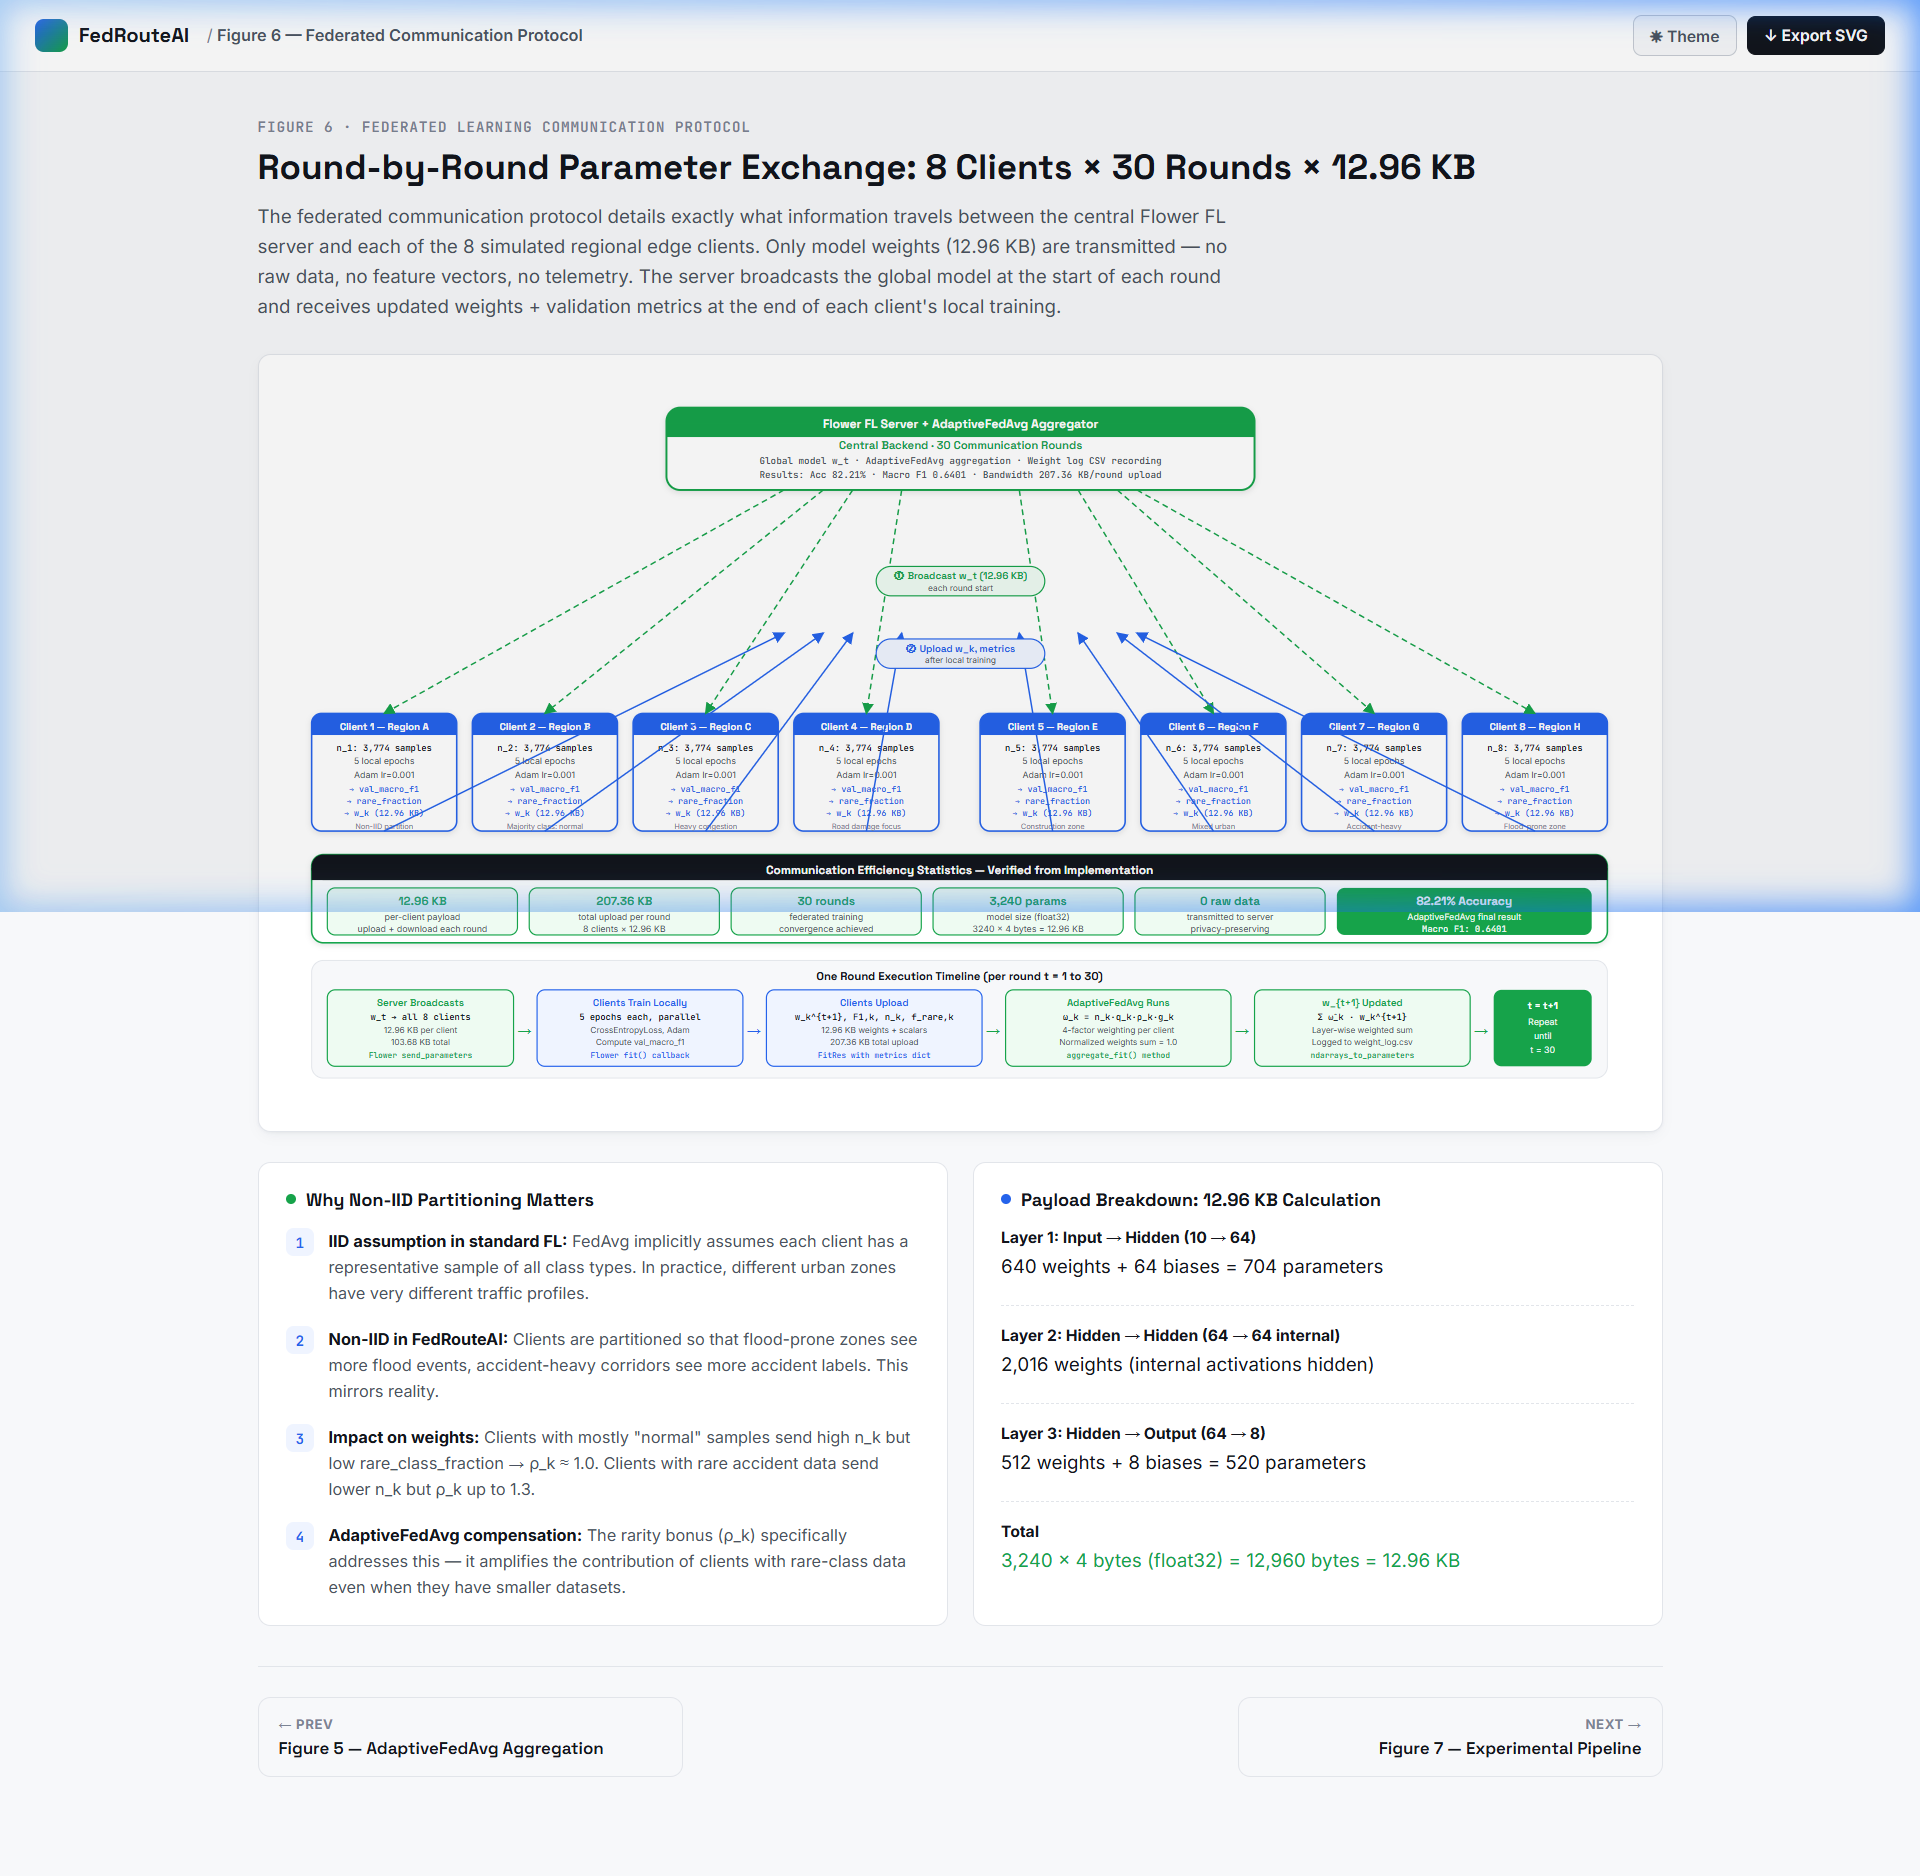
\includegraphics[width=0.95\textwidth]{figures/fig6_fl_communication.png}
  \caption{Federated learning communication protocol across 8 regional edge clients over 30 training rounds. The server broadcasts the global model $w_t$ (12.96\,KB) at each round start (green arrows) and receives updated weights plus validation metrics from all clients at round end (blue arrows). Total upload bandwidth per round: $8 \times 12.96 = 207.36$\,KB.}
  \label{fig:fl_communication}
\end{figure*}

\begin{algorithm}[htbp]
\caption{AdaptiveFedAvg Server Aggregation}
\label{alg:adaptivefedavg}
\begin{algorithmic}[1]
\REQUIRE Set of participating clients $\mathcal{K}$, Global model $w_t$, Round $t$, Parameters $\alpha, \beta, q_{floor}, g_{min}, \tau_{thresh}$
\ENSURE Updated global model $w_{t+1}$
\FOR{each client $k \in \mathcal{K}$ \textbf{in parallel}}
    \STATE $w_{t+1}^k \leftarrow \text{ClientUpdate}(k, w_t)$
    \STATE Evaluate validation Macro F1 $F_{1,k}$ and dataset size $n_k$
    \STATE Send $w_{t+1}^k, F_{1,k}, n_k$ to aggregation server
\ENDFOR
\STATE Server receives updates from all $k \in \mathcal{K}$
\FOR{each client $k \in \mathcal{K}$}
    \STATE Compute quality factor: $q_k = \max(q_{floor}, F_{1,k})$
    \STATE Compute rarity bonus: $\rho_k = 1.0 + \beta \cdot f_{rare}^k$
    \STATE Update F1 Exponential Moving Average:
    \STATE \quad $\text{EMA}_{F1}^k \leftarrow \alpha F_{1,k} + (1 - \alpha) \text{EMA}_{F1}^k$
    \IF{$\text{EMA}_{F1}^k \ge \tau_{thresh}$}
        \STATE $g_k \leftarrow 1.0$
    \ELSE
        \STATE $g_k \leftarrow g_{min} + (1.0 - g_{min}) \cdot \left(\frac{\text{EMA}_{F1}^k}{\tau_{thresh}}\right)$
    \ENDIF
    \STATE Calculate dynamic weight: $\omega_k = n_k \cdot q_k \cdot \rho_k \cdot g_k$
\ENDFOR
\STATE Normalize weights: $\hat{\omega}_k = \frac{\omega_k}{\sum_{j \in \mathcal{K}} \omega_j}$
\STATE Aggregate global parameters: $w_{t+1} \leftarrow \sum_{k \in \mathcal{K}} \hat{\omega}_k w_{t+1}^k$
\RETURN $w_{t+1}$
\end{algorithmic}
\end{algorithm}

